% Requires \usepackage{graphicx}
% Put the two PDFs in the same folder as your main .tex file,
% or use the relevant relative paths in \includegraphics.

\begin{figure}[tbp]
    \centering
    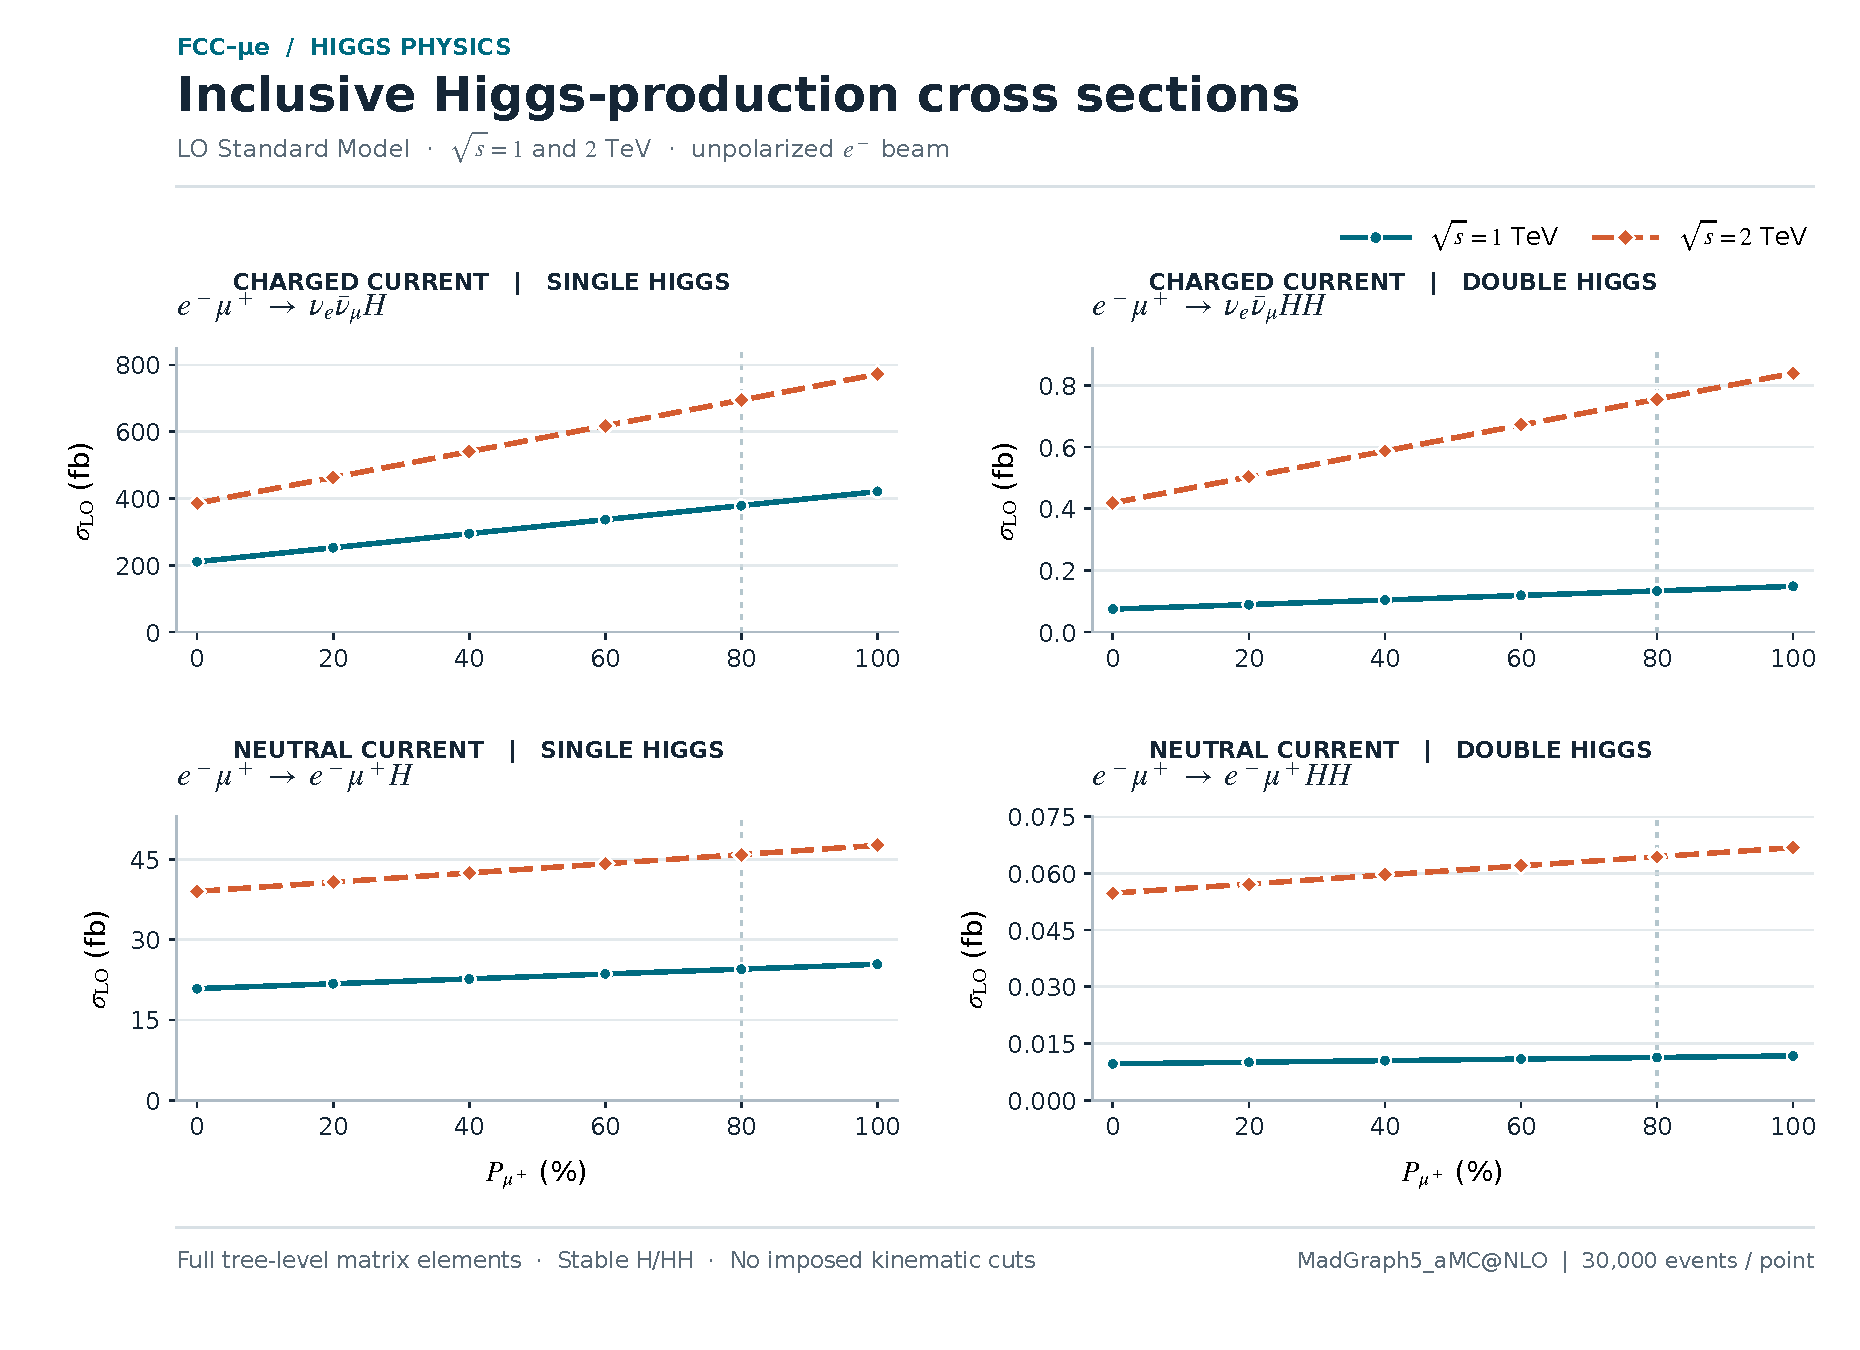
\includegraphics[width=\textwidth]{Figure_1_absolute_cross_sections.pdf}
    \caption{Leading-order Standard Model cross sections for inclusive single-
    and double-Higgs production in $e^-\mu^+$ collisions as functions of the
    positive-muon longitudinal polarization $P_{\mu^+}$.
    Charged-current (top) and neutral-current (bottom) final states are shown
    at $\sqrt{s}=1$ and $2\,\mathrm{TeV}$, with unpolarized electrons.
    The points are MadGraph results with Monte Carlo integration uncertainties;
    lines are weighted linear fits. Higgs bosons are kept stable and no
    kinematic generation cuts are imposed. The vertical guide indicates
    $P_{\mu^+}=80\%$.}
    \label{fig:FCCmue_absolute_cross_sections}
\end{figure}

\begin{figure}[tbp]
    \centering
    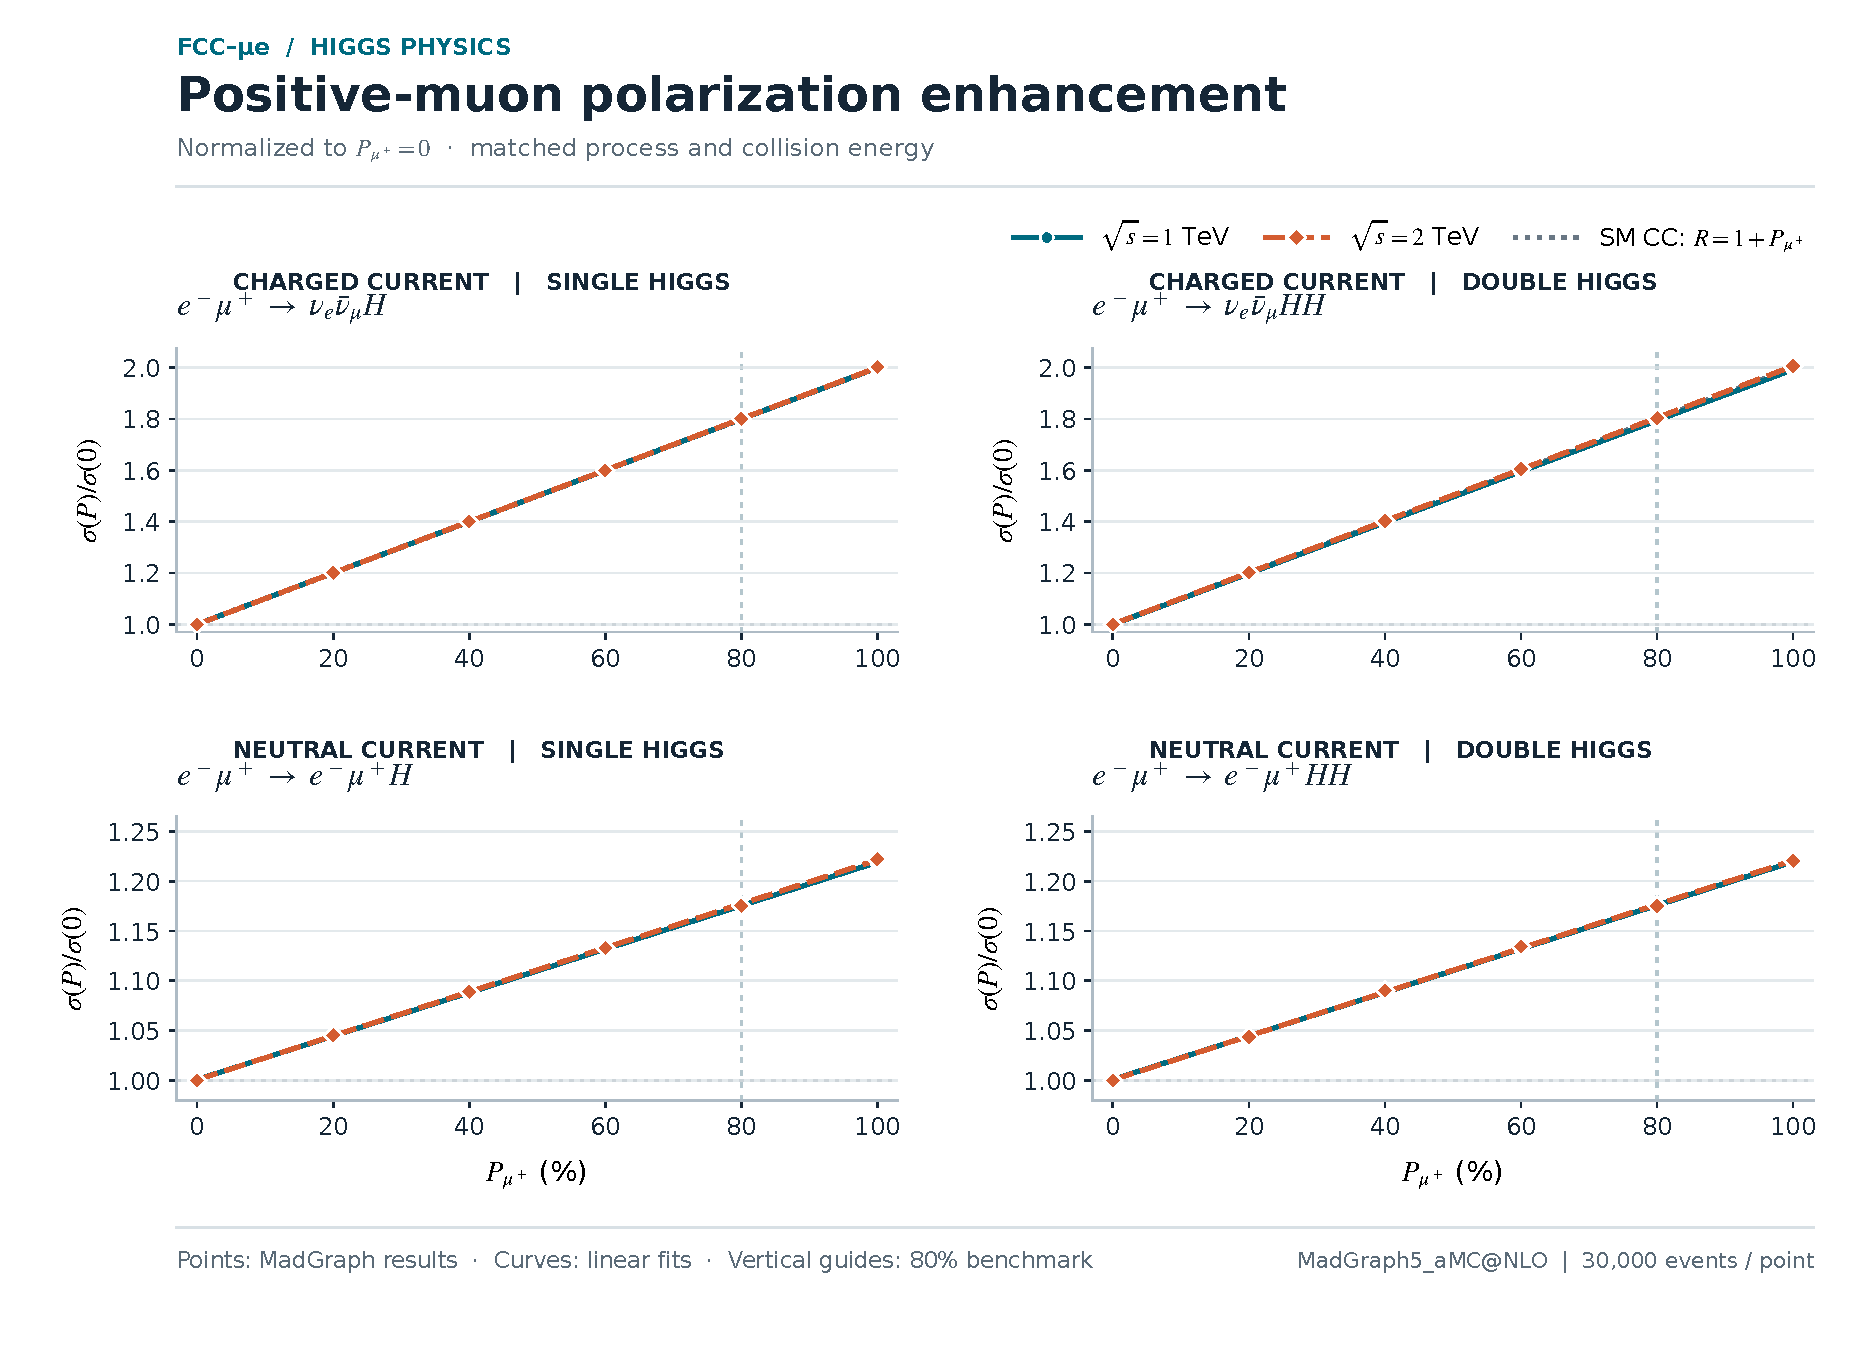
\includegraphics[width=\textwidth]{Figure_2_polarization_ratios.pdf}
    \caption{Polarization enhancement ratios
    $R(P_{\mu^+})=\sigma(P_{\mu^+})/\sigma(0)$ for the four Higgs-production
    channels at $\sqrt{s}=1$ and $2\,\mathrm{TeV}$.
    The charged-current results follow the Standard Model expectation
    $R\simeq1+P_{\mu^+}$ (with polarization expressed as a fraction),
    whereas the neutral-current enhancement is weaker.
    Points denote the Monte Carlo results, solid/dashed colored curves are
    linear fits, and the dotted reference line in the upper panels is the
    charged-current expectation. The electron beam is unpolarized.}
    \label{fig:FCCmue_polarization_ratios}
\end{figure}
